\renewcommand*{\arraystretch}{1.1}

\subsection*{BI / read / 25}
\label{section:bi-read-25}

% change \emph{} to use sans-serif font
\let\oldemph\emph
\renewcommand{\emph}[1]{{\footnotesize \sf #1}}

\renewcommand{\currentQueryCard}{25}
\marginpar{
	\raggedleft
	\vspace{0.22ex}

    \queryRefCard{bi-read-01}{BI}{1}\\
    \queryRefCard{bi-read-02}{BI}{2}\\
    \queryRefCard{bi-read-03}{BI}{3}\\
    \queryRefCard{bi-read-04}{BI}{4}\\
    \queryRefCard{bi-read-05}{BI}{5}\\
    \queryRefCard{bi-read-06}{BI}{6}\\
    \queryRefCard{bi-read-07}{BI}{7}\\
    \queryRefCard{bi-read-08}{BI}{8}\\
    \queryRefCard{bi-read-09}{BI}{9}\\
    \queryRefCard{bi-read-10}{BI}{10}\\
    \queryRefCard{bi-read-11}{BI}{11}\\
    \queryRefCard{bi-read-12}{BI}{12}\\
    \queryRefCard{bi-read-13}{BI}{13}\\
    \queryRefCard{bi-read-14}{BI}{14}\\
    \queryRefCard{bi-read-15}{BI}{15}\\
    \queryRefCard{bi-read-16}{BI}{16}\\
    \queryRefCard{bi-read-17}{BI}{17}\\
    \queryRefCard{bi-read-18}{BI}{18}\\
    \queryRefCard{bi-read-19}{BI}{19}\\
    \queryRefCard{bi-read-20}{BI}{20}\\
    \queryRefCard{bi-read-21}{BI}{21}\\
    \queryRefCard{bi-read-22}{BI}{22}\\
    \queryRefCard{bi-read-23}{BI}{23}\\
    \queryRefCard{bi-read-24}{BI}{24}\\
    \queryRefCard{bi-read-25}{BI}{25}\\
}


\noindent\begin{tabularx}{\queryCardWidth}{|>{\queryPropertyCell}p{\queryPropertyCellWidth}|X|}
	\hline
	query & BI / read / 25 \\ \hline
%
	title & Weighted interaction paths
 \\ \hline
%
	pattern & \hfill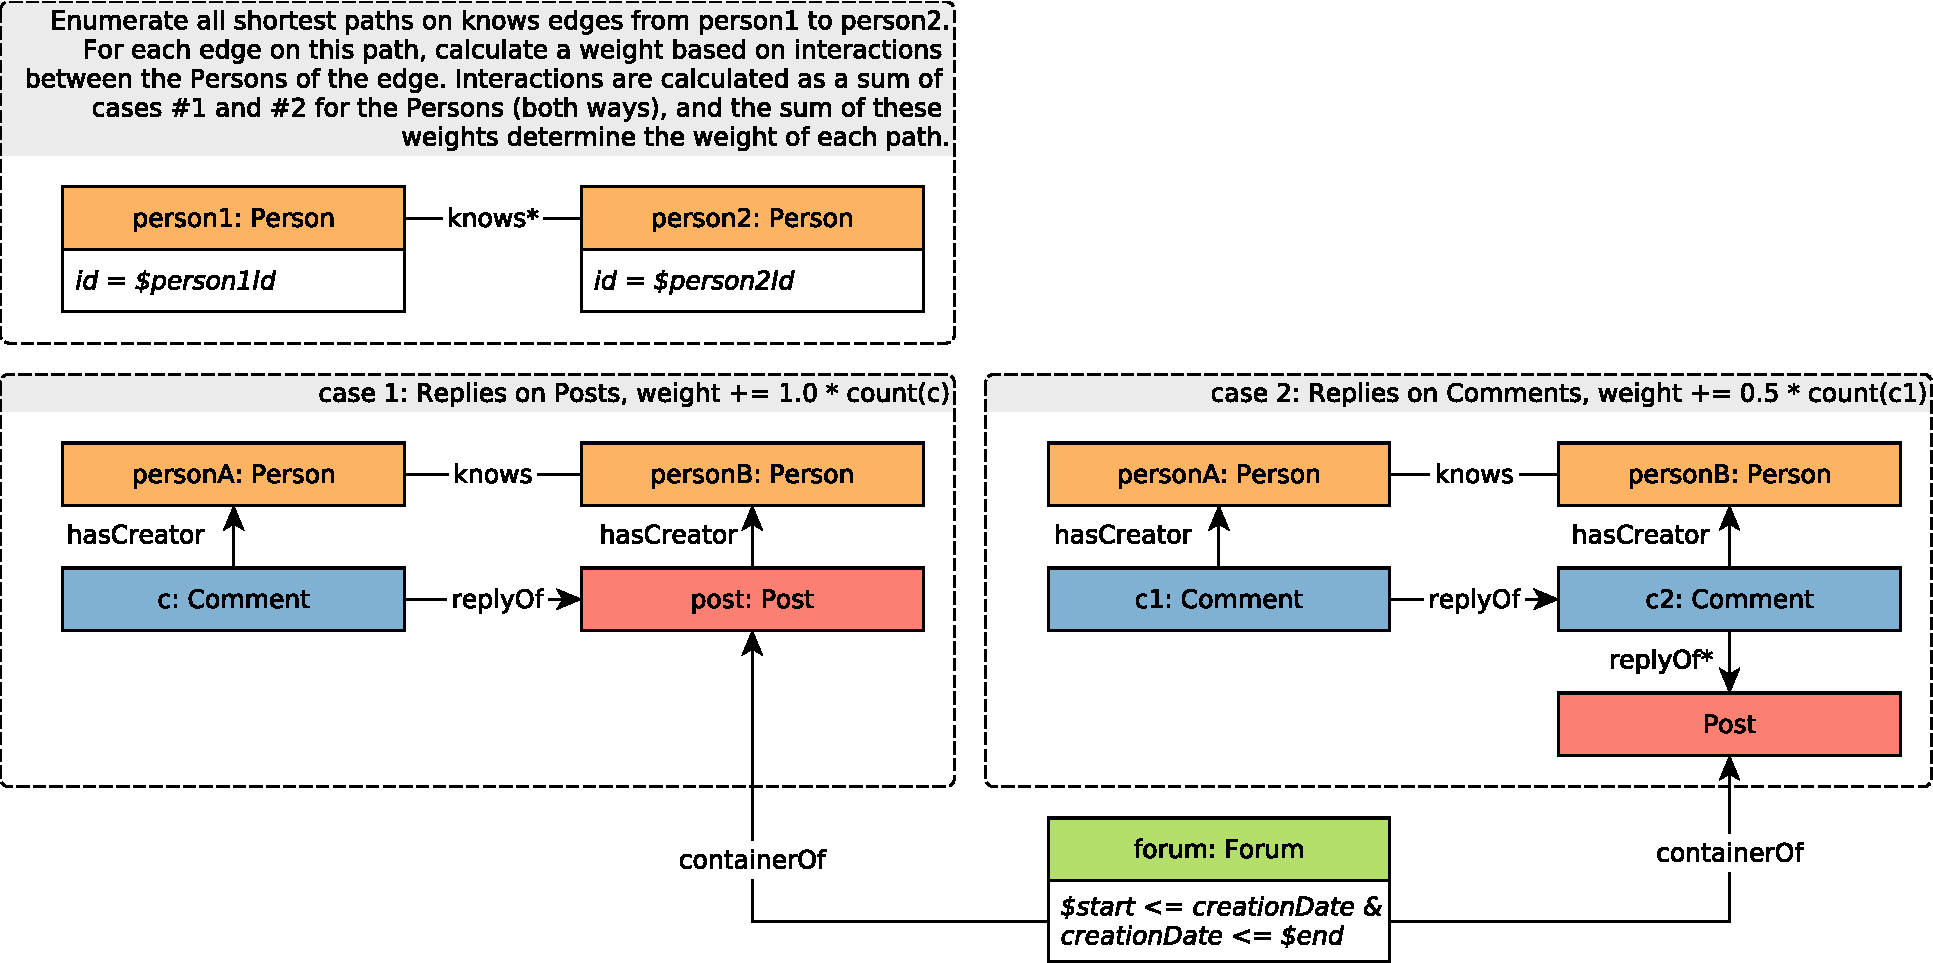
\includegraphics[scale=\patternscale,margin=0cm .2cm]{patterns/bi-read-25}\hfill\vadjust{} \\ \hline
%
	desc. & Given two \emph{Persons}, find all (unweighted) shortest paths between
these two \emph{Persons}, in the subgraph induced by the \emph{knows}
relationship.

Then, for each path calculate a weight. The nodes in the path are
\emph{Persons}, and the weight of a path is the sum of weights between
every pair of consecutive \emph{Person} nodes in the path.

The weight for a pair of \emph{Persons} is calculated based on their
interactions:

\begin{itemize}
\tightlist
\item
  Every reply (by one of the \emph{Persons}) to a \emph{Post} (by the
  other \emph{Person}) contributes 1.0.
\item
  Every reply (by one of the \emph{Persons}) to a \emph{Comment} (by the
  other \emph{Person}) contributes 0.5.
\end{itemize}

Only consider \emph{Messages} that were created in a \emph{Forum} that
was created within the timeframe \texttt{{[}startDate,\ endDate{]}}.

Return all the paths with shortest length, and their weights.
 \\ \hline
%
	
		params &
		\innerCardVSpace{\begin{tabularx}{\attributeCardWidth}{|>{\paramNumberCell}c|>{\varNameCell}M|>{\typeCell}m{\typeWidth}|Y|} \hline
		$\mathsf{1}$ & person1Id
 & 64-bit Integer
 &  \\ \hline
		$\mathsf{2}$ & person2Id
 & 64-bit Integer
 &  \\ \hline
		$\mathsf{3}$ & startDate
 & Date
 &  \\ \hline
		$\mathsf{4}$ & endDate
 & Date
 &  \\ \hline
		\end{tabularx}}\innerCardVSpace \\ \hline
	
%
	
		result &
		\innerCardVSpace{\begin{tabularx}{\attributeCardWidth}{|>{\resultNumberCell}c|>{\varNameCell}M|>{\typeCell}m{\typeWidth}|>{\resultOriginCell}c|Y|} \hline
		$\mathsf{1}$ & person.id & 64-bit Integer{[}{]} & R &
				Identifiers representing an ordered sequence of the \emph{Persons} in
the path weight
 \\ \hline
		\end{tabularx}}\innerCardVSpace \\ \hline
	
%
	
		sort		&
		\innerCardVSpace{\begin{tabularx}{\attributeCardWidth}{|>{\sortNumberCell}c|>{\varNameCell}M|>{\directionCell}c|Y|} \hline
		$\mathsf{1}$ & weight
 & $\desc
$ & The order of paths with the same weight is unspecified
 \\ \hline
		\end{tabularx}}\innerCardVSpace \\ \hline
	%
	%
	CPs &
	\multicolumn{1}{>{\raggedright}l|}{
		\chokePoint{1.2}, 
		\chokePoint{2.1}, 
		\chokePoint{2.2}, 
		\chokePoint{2.4}, 
		\chokePoint{3.3}, 
		\chokePoint{5.1}, 
		\chokePoint{5.3}, 
		\chokePoint{7.2}, 
		\chokePoint{7.3}
		} \\ \hline
	%
	%
\end{tabularx}
\queryCardVSpace

% change \emph back to the old one
\renewcommand{\emph}[1]{\oldemph{#1}}